\documentclass[fontsize=11pt]{article}

\usepackage{multicol}
\usepackage{blindtext}
\usepackage{hyperref}
%\usepackage{layout}
%\usepackage{showframe}
%\usepackage[top=1in, bottom=1.25in, left=1.25in, right=1.25in]{geometry}
\usepackage[margin=1in]{geometry}
\usepackage{graphicx,calc}
%\usepackage{wrapfig}
\usepackage{cleveref}

\crefname{enumi}{step}{steps}


\renewcommand{\abstractname}{The ``elevator pitch"}

\tolerance=1
\emergencystretch=\maxdimen
\hyphenpenalty=9000
\hbadness=9000

\begin{document}

\raggedright
\pagenumbering{gobble}

\title{\huge{It's time for a refresh!} \\ \small{Resetting Firefox to a new, clean, and sane state} }
\author{Alan Amesbury\thanks{Thanks to my parents for inspiring this article.  Thanks to Cat for the second set of eyes and the copious amounts of red ink and yellow highlighter she applied to early versions.  Tech support remains open.}}
\date{January 2019}


\maketitle

\begin{abstract}{Over time, Firefox can accumulate information contained in user profiles that might make it less stable or slow it down.  Firefox's creators provided a \emph{refresh} feature to fix this problem.  This article tells you how you can use this feature, and includes additional steps you can take to also improve your online experience by making browsing the web safer and faster.}
\end{abstract}

%\begin{multicols}{2}



%%%%%%%%%%%%%%%%%%%%%%%%%%%%%%%%%%%%%%%%%%%%%%%
%%%%%%%%%%%%%%%%%%%%%%%%%%%%%%%%%%%%%%%%%%%%%%%
\section{``Refresh" overview}
Firefox stores information in a \emph{user profile}.  Your user profile includes things like your bookmarks, passwords you've asked Firefox to save, and much more.  As Firefox is updated over time, the format in which this data is kept can also change.  Firefox's creators try to make updates a painless experience for Firefox users and hide a lot of the technical details that almost all users would find uninteresting, so many changes (often even major ones) are usually invisible to anyone who isn't deliberately looking for them.

If you're reading this, you likely fall into the category of people who are less interested in those details and more interested in having things \underline{just~work}, and it's for you that Mozilla created the ``refresh" option.  This feature of Firefox does several things, including:
\begin{itemize}
	\item{Removes website permissions, which websites may use your camera and microphone}
	\item{Resets preference settings, such as your preferred home page or default search engine}
	\item{Removes extensions and themes that aren't part of Firefox (including ones that may have been installed without you realizing it)}
\end{itemize}


Some of the things a refresh does \emph{not} change or reset are:
\begin{itemize}
	\item{Bookmarks}
	\item{Passwords stored in the browser}
	\item{Browsing history}
\end{itemize}


Bottom line:  Refreshing Firefox takes you as close to ``clean slate" as Firefox can get without also erasing important things like your bookmarks.  It is also completely safe for all your other data, because Firefox's refresh doesn't change anything else.





%%%%%%%%%%%%%%%%%%%%%%%%%%%%%%%%%%%%%%%%%%%%%%%
%%%%%%%%%%%%%%%%%%%%%%%%%%%%%%%%%%%%%%%%%%%%%%%
\section{Just the refresh, please!}\label{section:just-the-refresh-please}

\begin{figure}[h]
	\centering
	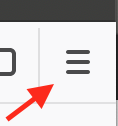
\includegraphics{images/hamburger-menu.png}
	\caption{The menu button}
	\label{fig:hamburger-menu}
\end{figure}

If all you want to do is return Firefox to a state as close as it can be to a clean installation without erasing your bookmarks, browsing history, etc., there's very little you need to do.  First, find and click the ``menu" button\footnote{Some software and web developers call this the ``hamburger menu."}  A picture of it is shown in \cref{fig:hamburger-menu}.

From this menu, open ``Help" and select ``Troubleshooting Information."  (If you prefer to open this page directly, you can also reach it directly using the URL \texttt{about:support}.\footnote{Many Firefox configuration pages can be reached in more than one way.  You can use whichever is easiest for you.})  Near the top of the page is a button labeled ``Refresh Firefox\ldots{}"  Clicking it causes Firefox to confirm that's what you actually want to do.  Once you confirm the action, Firefox restarts.

After restart, Firefox may ask about restoring windows or tabs you might have had open when you did the refresh.  Choose whichever option you want.  Also, Firefox saves your settings from before the refresh in a folder on your desktop.  This can be used to restore things to the way they were before the refresh or, if you're happy with the results, discarded.  (See \cref{section:undo-the-refresh} for details.)




%%%%%%%%%%%%%%%%%%%%%%%%%%%%%%%%%%%%%%%%%%%%%%%
%%%%%%%%%%%%%%%%%%%%%%%%%%%%%%%%%%%%%%%%%%%%%%%
\section{Just the refresh\ldots{}but what about extensions I want to keep?}
Firefox removes extensions when you do a refresh, which means you'll need to reinstall them if you still want them.  To do that, you'll need to know which extensions are installed \emph{before} you do a refresh.  This list is available from the \texttt{about:support} page (described in \cref{section:just-the-refresh-please}), but you can also view it by clicking the menu button and selecting ``Add-ons."  You'll need to record these somewhere so you know which ones to install after you refresh Firefox.  Keep in mind this is also an excellent time to decide what extensions you really want to keep.  See one you don't recognize?  You may not actually want it!

After you have the list of extensions you want to continue using after the refresh, it's time to refreh Firefox.  (See \cref{section:just-the-refresh-please} for details on how to do that.). When the refresh is complete, it's time to install the extensions you want.





%%%%%%%%%%%%%%%%%%%%%%%%%%%%%%%%%%%%%%%%%%%%%%%
%%%%%%%%%%%%%%%%%%%%%%%%%%%%%%%%%%%%%%%%%%%%%%%
\section{(Re)installing extensions}



\subsection{General information}

\begin{figure}[h]
	\centering
	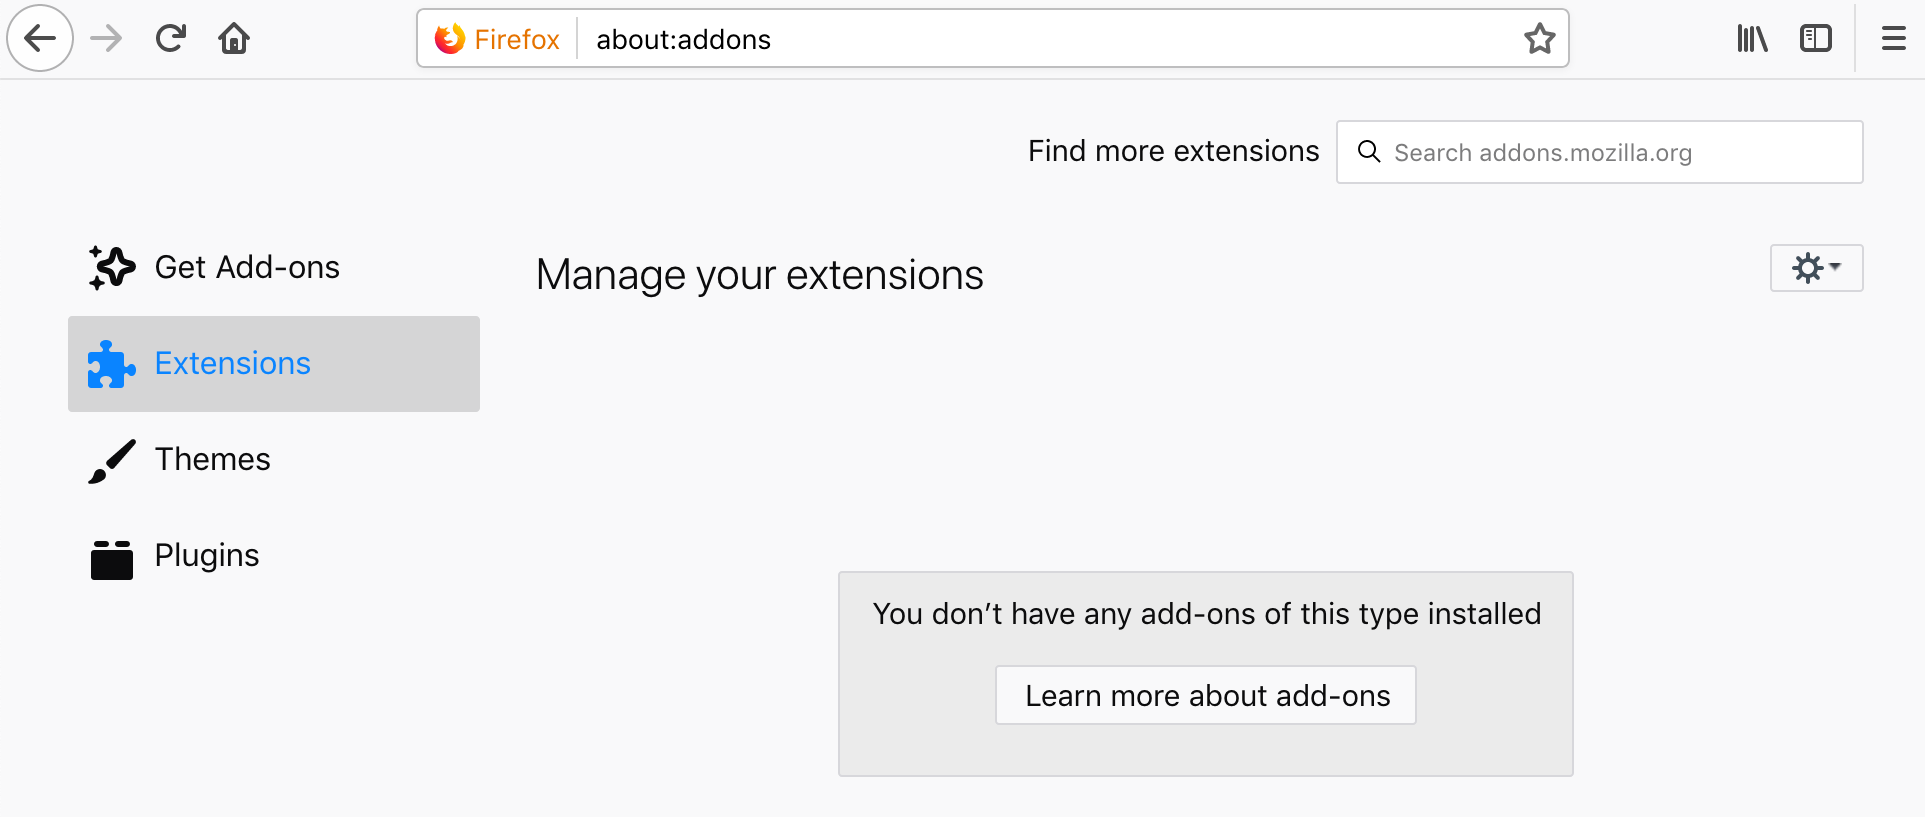
\includegraphics[width=0.85\textwidth]{images/extensions-post-refresh.png}
	\caption{The extensions manager post-refresh }
	\label{fig:extensions-post-refresh}
\end{figure}

Extensions are add-ons you can install that extend Firefox's basic functionality.  To install extensions, go to the \texttt{about:addons} page, or click the menu button and select ``Add-ons."  Next, select ``Extensions" from the list at the left.  In the ``Find more extensions" box, type the name of an extension you want to install.  Note that extensions that are already installed will appear here; the list should be empty\footnote{Since Firefox changes more quickly than this article, it's possible that extensions may someday be included post-refresh.  Howver, since the point of a refresh is to clear out old extensions, anything remaining should be examined to ensure that it actually belongs there, e.g., it's something placed there by Firefox's creators.} after refreshing Firefox.  See \cref{fig:extensions-post-refresh} for an example of what this screen should\footnote{This is from a Mac.  Windows systems may look a bit different.} look like.




\subsection{Suggested extensions}
Firefox has thousands of extensions (at least!), so providing a list of \emph{all} the useful ones would be an impossible task.  However, many people find these few to be particularly useful:

\begin{itemize}
	\item uBlock Origin
	\item HTTPS Everywhere
	\item Privacy Badger
\end{itemize}


\subsubsection{uBlock Origin}
 uBlock Origin provides the ability to block a variety of content many people find annoying or troublesome, including ads and some malicious content.  It is highly configurable, but has default settings that most people should find work for them.  While it can function like extensions explicitly designed to block ads, this is not its sole purpose.  If you are  opposed to blocking ads, you may disable this functionality while keeping other features (like the malware protection) active.

 If you only install one extension, this is the one to install.


\subsubsection{Privacy Badger}
The Electronic Frontier Foundation (EFF) is a non-profit group known for its interests in digital privacy and free speech.  It's helped to develop tools people can use to defend their privacy online, and one of those tools is Privacy Badger.  This extension is designed specifically to help prevent websites from surreptitiously tracking your activity.  While some of its functionality is duplicated in uBlock Origin, Privacy Badger differs fundamentally in how it works.  This means it may still protect you in situations wheree uBlock Origin might not.  Read the EFF's excellent FAQ on Privacy Badger at https://www.eff.org/privacybadger.


\subsubsection{HTTPS Everywhere}
 EFF also created HTTPS Everywhere.  It attempts to force your web browser to use HTTPS, the encrypted form of web communication, when it connects to websites.  Although many major sites (Google, Youtube, Twitter, etc.) have shifted their default communications to HTTPS by default, this extension still has value because it attempts to use encryption even for websites that haven't yet made that leap.



\section{Other things to consider}
There are a couple other things you can do to Firefox following a refresh that may help improve your security with almost no chance of interfering with normal operation.  There are actually a lot of things you \emph{could} change here, but these are the few that are really worth considering whether you \emph{should} change.

\subsection{Changes to consider in Firefox's default preferences}
Click the menu button, open ``Preferences" (if you're using macOS) or ``Options" (if you're using WIndows).


\begin{itemize}
	\item Select the ``Home" section on the left, then scroll down to the ``Firefox Home Content" section.  Do you use Pocket?  If not, disable it and the ``Sponsored Stories" option.  Are you interested in seeing news updates\footnote{These have nothing to do with keeping Firefox itself up to date.} about Mozilla and Firefox?  If not, turn off ``Snippets."

	\item Select the ``Search" section on the left, then scroll down to the ``Default Search Engine" section.  Do you want to use the default provided?  If not, choose something else.  Do you want that search engine to see everything you enter for a search before you send it so it can attempt to guess what you're searching for?  If not, turn off ``Provide search suggestions."

	\item Select the ``Privacy \& Security" section on the left, then scroll down to ``Logins \& Passwords."  Do you want your browser to save usernames and passwords that you enter into it?  If not, turn off ``Ask to save logins and passwords for websites."  If you \emph{do} want to use this feature and share your computer with family or friends, consider enabling ``Use a master password."  This will help prevent someone else from being able to access your saved credentials.  Note that losing the master password will likely mean you also lose access to whatever it protects.

	\item Scroll down to ``Permissions."  By default Firefox lets a couple of websites install extensions with minimal permission from you.  Click on the ``Exceptions\ldots{}" button next to ``Warn you when websites try to install add-ons," remove all websites shown, and save your changes.  Make sure the checkbox next to ``Warn you when websites try to install add-ons" remains checked.

	\item Scroll down to ``Firefox Data Collection and Use."  Do you want Firefox to send technicaal information and information about your activities to Mozilla so they can analyze it?  If not, turn this off.
\end{itemize}



\subsection{Other changes to consider (bonus round!)}
Firefox includes a large number of other configuration options that aren't available through ``Preferences" or ``Options'' menus.  To access these, type \texttt{about:config} in the address bar.  This will display a scary warning (an exclamation symbol with ``This might void your warranty!"), but in a worst-case scenario you can just refresh Firefox to recover from a botched attempt to make changes.  \emph{The warning does not mean data on your computer is at risk when you make configuration changes.}  Unless you're careless, it's unlikely you'll cause problems from which you can't recover.  Click ``I accept the risk!" to open the list of configuration options.

\begin{figure}[h]
	\centering
	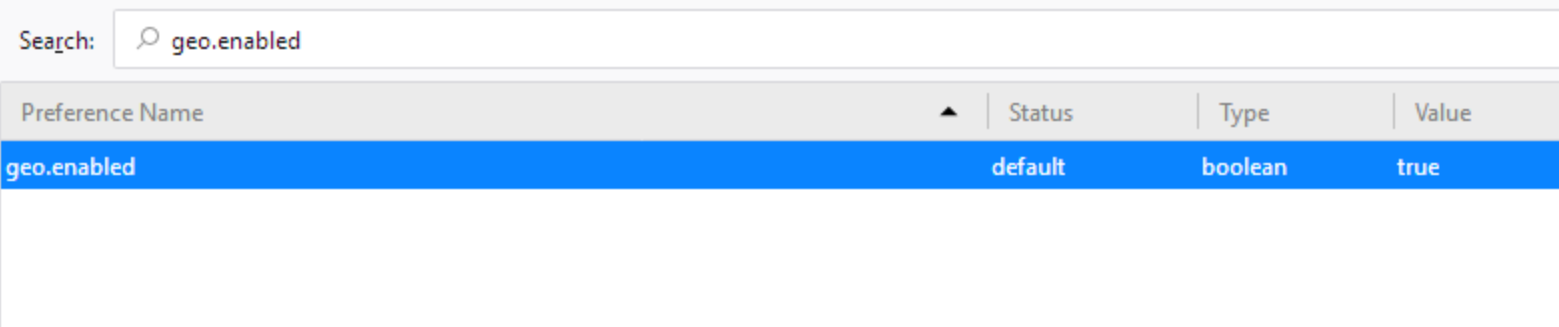
\includegraphics[width=0.85\textwidth]{images/about-config.png}
	\caption{The \texttt{geo.enabled} option on the \texttt{about:config} page}
	\label{fig:about-config}
\end{figure}

If you do not want Firefox to \emph{ever} provide your location to a website, you can disable this feature by setting the \texttt{geo.enabled} option to ``false."  First, find the option by entering ``geo.enabled" in the search box on the \texttt{about:config} page.  Toggle between ``true" (the default setting) and ``false" by double clicking the option.  Disabling it will not only prevent Firefox from sharing your location, it will stop it from asking for permission every time a website requests it.  See \cref{fig:about-config} for an example of what this looks like.



Firefox includes support for older cryptography because a few websites still use it.  Most websites, however, have moved on, so most people don't really need support for the older stuff.  Disabling support for it in Firefox improves security with little risk of breaking things and, if disabling it does cause problems, it's easy to reverse the change.\footnote{If you're interested in the details, this is about TLS support in Firefox.  By default it supports TLSv1, which has known weaknesses.  The recommendation here is to disable support for versions older than TLS v1.2.}

Type ``security.tls.version.min" in the search box on the \texttt{about:config} page, then double click the ``security.tls.version.min" option.  This opens a box asking for an ``integer value."  Enter a ``3" to force Firefox to only use newer, secure cryptography and click ``OK."  If you encounter problems with a website and think changing this setting is the cause, you can change it back to its original value (``1" as of January, 2019).


\section{I want to undo the refresh!}\label{section:undo-the-refresh}
When Firefox does a refresh, it saves all your previous settings in a folder called ``Old Firefox Data" on your desktop.  Undoing a refresh is not as easy as the refresh, but recovery is still possible.  The details of what to do differ somewhat between macOS and Windows, but the idea is to copy the old data over the new user profile Firefox created when you did the refresh.

Here's what you do:
\begin{enumerate}
	\item Find the ``Old Firefox Data" folder on your desktop, but don't open it yet.
	\item Open the \texttt{about:support} page in Firefox.
	\item \label{step:open-profile} In the ``Application Basics" section, find the line containing ``Profile Folder."  Press the button on that line labeled ``Show in Finder'' (on macOS) or ``Open folder" (on Windows) to open the folder containing your current user profile.  This is the one we're going to replace.
	\item Close Firefox completely and make sure it is not running.
	\begin{itemize}
		\item On macOS you can verify this by checking the Dock.  If the Firefox icon is not present, Firefox isn't running.  If it is present, click and hold on the icon until a menu pops up.  If ``Quit" is an option in the menu, select it.  If ``Quit" is not an option, it means Firefox isn't running.  You can click anywhere else on the screen to close the pop-up menu.
		\item On Windows you can verify Firefox is closed by checking the Task Manager.  Holding the ``Alt" and ``Control" keys, press the ``Delete" key, then select ``Task Manager" from the available options.  If Firefox is not shown in the list of running applications or processes, it isn't running.  If it is running, select it from the list of applications or processes, then click the ``End task" button.  Close Task Manager when you're done.
	\end{itemize}
	\item On Windows, Firefox opened only the active profile folder in \cref{step:open-profile}.  On macOS it opened the folder containing profile folders, and there may be more than one.  If this is true in your case, open the one that has the word ``default" in it.  If more than one has folder contains ``default," open the one that was modified most recently.  You may need to view this window as a list (open Finder's ``View" menu and select ``as List") to see this information.
	\item You should now be looking at a folder with a weird, mostly unpronouceable name like ``knsklwk.default" or ``enknakjei.default-1573829300" containing a bunch of files and folders.  Select all of the files and folders within that folder and drag them to the trash (recycle bin on Windows).  This should leave you an empty folder with a weird name.
	\item Open the ``Old Firefox Data" folder you located earlier.
	\item Select all items in the folder.
	\item Copy them to the profile folder with the weird name.  This is \emph{not} the same as simply dragging them from one place to another, as this will usually move them, not copy them.  You want to copy them instead of moving them in case something goes wrong and you need to restart this procedure.
	\item Close both folders.
	\item Start Firefox.
\end{enumerate}

At this point Firefox is running using the data you copied from the backup it made of your user profile when you did the refresh, competely reversing the refresh.



\section{Resources}
Hopefully after following at least some of these instructions you've wound up with a better performing and more secure browser, and also fixed any problems you might've been having that led you here in the first place.  Additional information and help can be found at these and other locations online:
\begin{itemize}
	\item For Firefox itself:
	\begin{itemize}
		\item https://support.mozilla.org/products/firefox
	\end{itemize}
	Recovering old Firefox profile data:
	\begin{itemize}
		\item https://support.mozilla.org/en-US/kb/recovering-important-data-from-an-old-profile
	\end{itemize}
	\item For extensions mentioned here:
	\begin{itemize}
		\item https://addons.mozilla.org/firefox/addon/ublock-origin/ (\mbox{uBlock Origin})
		\item https://www.eff.org/privacybadger (\mbox{Privacy Badger})
		\item https://www.eff.org/https-everywhere (\mbox{HTTPS Everywhere})
	\end{itemize}
\end{itemize}

%\end{multicols}

\end{document}